\documentclass{article}

\usepackage{fancyhdr}
\usepackage{extramarks}
\usepackage{amsmath}
\usepackage{amsthm}
\usepackage{amsfonts}
\usepackage{tikz}
\usepackage[plain]{algorithm}
\usepackage{algpseudocode}
\usepackage{enumerate}
\usepackage{mathtools}
\usepackage{forest}
\usepackage{adjustbox}
\usepackage[table]{colortbl}
\usepackage{graphicx}
\graphicspath{ {images/} }

\usetikzlibrary{automata,positioning}

%
% Basic Document Settings
%

\topmargin=-0.45in
\evensidemargin=0in
\oddsidemargin=0in
\textwidth=6.5in
\textheight=9.0in
\headsep=0.25in

\linespread{1.1}

\pagestyle{fancy}
\lhead{\hmwkAuthorName}
\chead{\hmwkClass\ (\hmwkClassInstructor\ \hmwkClassTime): \hmwkTitle}
\rhead{\firstxmark}
\lfoot{\lastxmark}
\cfoot{\thepage}

\renewcommand\headrulewidth{0.4pt}
\renewcommand\footrulewidth{0.4pt}

\setlength\parindent{0pt}

%
% Create Problem Sections
%

\newcommand{\enterProblemHeader}[1]{
    \nobreak\extramarks{}{Problem \arabic{#1} continued on next page\ldots}\nobreak{}
    \nobreak\extramarks{Problem \arabic{#1} (continued)}{Problem \arabic{#1} continued on next page\ldots}\nobreak{}
}

\newcommand{\exitProblemHeader}[1]{
    \nobreak\extramarks{Problem \arabic{#1} (continued)}{Problem \arabic{#1} continued on next page\ldots}\nobreak{}
    \stepcounter{#1}
    \nobreak\extramarks{Problem \arabic{#1}}{}\nobreak{}
}

\setcounter{secnumdepth}{0}
\newcounter{partCounter}
\newcounter{homeworkProblemCounter}
\setcounter{homeworkProblemCounter}{1}
\nobreak\extramarks{Problem \arabic{homeworkProblemCounter}}{}\nobreak{}

%
% Homework Problem Environment
%
% This environment takes an optional argument. When given, it will adjust the
% problem counter. This is useful for when the problems given for your
% assignment aren't sequential. See the last 3 problems of this template for an
% example.
%
\newenvironment{homeworkProblem}[1][-1]{
    \ifnum#1>0
        \setcounter{homeworkProblemCounter}{#1}
    \fi
        \section{Problem \arabic{homeworkProblemCounter}}
    \setcounter{partCounter}{1}
    \enterProblemHeader{homeworkProblemCounter}
}{
    \exitProblemHeader{homeworkProblemCounter}
}

%
% Homework Details
%   - Title
%   - Due date
%   - Class
%   - Section/Time
%   - Instructor
%   - Author
%

\newcommand{\hmwkTitle}{Homework \#8}
\newcommand{\hmwkDueDate}{April 14, 2016}
\newcommand{\hmwkClass}{CS 373}
\newcommand{\hmwkClassInstructor}{Professor David Garrison}
\newcommand{\hmwkClassTime}{Section B1}
\newcommand{\hmwkAuthorName}{Tim Hung}

%
% Title Page
%

\title{
    \vspace{2in}
    \textmd{\textbf{\hmwkClass:\ \hmwkTitle}}\\
    \normalsize\vspace{0.1in}\small{Due\ on\ \hmwkDueDate\ at 2:20pm}\\
    \vspace{0.1in}\large{\textit{\hmwkClassInstructor\ \hmwkClassTime}}\\
}

\author{\textbf{\hmwkAuthorName}}
\date{}

\renewcommand{\part}[1]{\textbf{\large Part \Alph{partCounter}}\stepcounter{partCounter}\\}

%
% Various Helper Commands
%

% Useful for algorithms
\newcommand{\alg}[1]{\textsc{\bfseries \footnotesize #1}}

% For derivatives
\newcommand{\deriv}[1]{\frac{\mathrm{d}}{\mathrm{d}x} (#1)}

% For partial derivatives
\newcommand{\pderiv}[2]{\frac{\partial}{\partial #1} (#2)}

% Integral dx
\newcommand{\dx}{\mathrm{d}x}

% Alias for the Solution section header
\newcommand{\solution}{\textbf{\large Solution}}

% Probability commands: Expectation, Variance, Covariance, Bias
\newcommand{\E}{\mathrm{E}}
\newcommand{\Var}{\mathrm{Var}}
\newcommand{\Cov}{\mathrm{Cov}}
\newcommand{\Bias}{\mathrm{Bias}}

\begin{document}

\maketitle

\pagebreak

\begin{homeworkProblem} 

    \begin{figure}
        \centering
        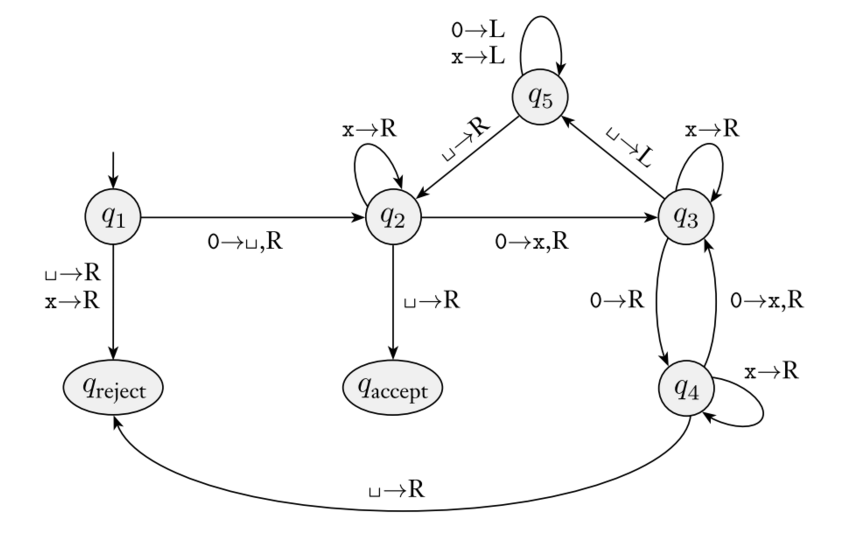
\includegraphics[width=\textwidth]{TM_M2}
        \caption{State diagram for Turing machine $M_2$}
    \end{figure}

    \textbf{(a)}    Give the sequence of configurations that $M_2$ enters when started on the input string '0'.
    \[
        q_1 0 
        \Rightarrow \sqcup q_2 \sqcup 
        \Rightarrow \sqcup \sqcup q_{\text{accept}}
    \]
    
    \textbf{(c)}    Give the sequence of configurations that $M_2$ enters when started on the input string '000'.
    \[
        q_1 000
        \Rightarrow \sqcup q_2 00
        \Rightarrow \sqcup xq_30
        \Rightarrow \sqcup x0q_4\sqcup
        \Rightarrow \sqcup x0\sqcup q_{\text{reject}}
    \]
\end{homeworkProblem}

\pagebreak

\begin{homeworkProblem} 
    \begin{figure}
        \centering
        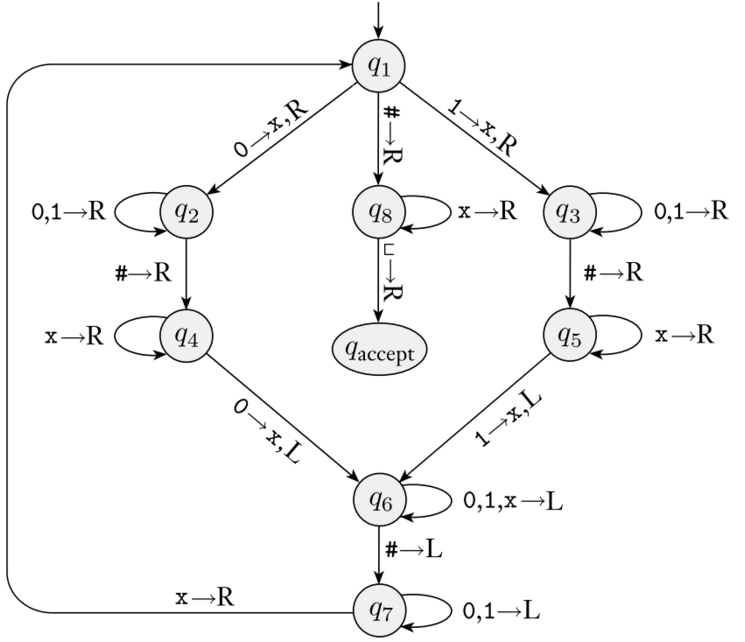
\includegraphics[width=\textwidth]{TM_M1}
        \caption{State diagram for Turing machine $M_1$}
    \end{figure}
    \textbf{(b)}    Give the sequence of configurations that $M_1$ enters when started on the input string '1\#1'.
    \[
        q_11\#1
        \Rightarrow x q_3\#1
        \Rightarrow x \# q_5 1
        \Rightarrow x q_5 \# x
        \Rightarrow q_5 x \# x
        \Rightarrow x q_1 \# x
        \Rightarrow x \# q_8 x
        \Rightarrow x \# x q_8
        \Rightarrow x \# x q_{accept}
    \]

    \textbf{(c)}    Give the sequence of configurations that $M_1$ enters when started on the input string '1\#\#1'.
    \[
        q_11\#\#1
        \Rightarrow x q_3\#\#1
        \Rightarrow x\#q_5\#1
        \Rightarrow x\#q_{5reject}\#1
    \]

\end{homeworkProblem}

\pagebreak

\begin{homeworkProblem} 
    Describe a Turing machine, sequence of steps, that recognizes $\{w|w\in\{a, b, c\}^*$ such that the number of a's in w $<$ the number of b's in w and the number of a's in w = the number of c's in w $\}$.\\

    \textbf{Solution}
    \begin{verbatim}
    A.  Push a $ to the left end of the tape and shift everyone to the right one
    B.  Scan from the left end to the first blank space
        1.  mark the first (b) with a #
            I.  if there's no unmarked (b), halt and reject
        2.  go back to the left end
    C.  Scan from the left end to the first blank space
        1.  mark the first (a) with a #
            I.  if there's no unmarked (a) continue, but remember that
        2.  go back to the left end
    D.  Scan from the left end to the first blank space
        1.  mark the first (c) with a #
            I.  if there's no unmarked (c)
                i.  if there was no unmarked (a) earlier, halt and accept
                ii. if there was a marked (a), halt and accept
        2.  go back to the left end
    E.  GOTO(B.) and repeat
    \end{verbatim}

\end{homeworkProblem}

\pagebreak

\begin{homeworkProblem} 
    A 2-PDA is a PDA with two stacks. In this problem we want to kind of show that a 2-PDA is as
    powerful as a Turing machine. 

    To do this, show the equivalent transitions for a 2-PDA for the Turing machine transitions $(q_i, X) \rightarrow (q_j, A, L)$ and $(q_i, X) \rightarrow (q_j, A, R)$ (in state $q_i$ read X, write A,
    and move left or right and transition to state $q_j$). 

    The transitions for a 2-PDA are of the form $(q_i,X, S_1, S_2) \rightarrow (q_j, T_1, T_2)$ (in state $q_i$, read X, pop $S_1$ from stack 1, pop $S_2$ from stack 2, transition to state $q_j$, push $T_1$ onto stack 1 and push $T_2$ onto stack 2). You don't have to prove the transitions are equivalent, just tell me what they are.\\

    In this problem we want the 2-PDAs first stack to represent the contents of the tape to the left of
    the Turing machine's read/write head and the second stack to represent the contents of the
    tape under the Turing machine's read/write head and to the right of the read/write head. Once
    we visualize it this way, it should be fairly obvious that a 2-PDA can accept any language that a
    Turing machine can as long as we can duplicate the two Turing machine transitions (left move
    and right move).\\

    To correctly initialize the second stack of the 2-PDA we simply read the input and push it into
    the first stack and then pop everything out of the first stack while pushing onto the second
    stack. Once we have done this, the first stack is empty and the second stack contains the input
    in the correct order.\\

    \textbf{Solution}

    Turing machine transition $(q_i, X) \rightarrow (q_j, A, L)$ is equivalent to the 2-PDA transition:

    $(q_i,X, S_1, \epsilon) \rightarrow (q_j, \epsilon, S_1)$\\

    Turing machine transition $(q_i, X) \rightarrow (q_j, A, R)$ is equivalent to the 2-PDA transition:

    $(q_i,X,\epsilon, S_2) \rightarrow (q_j, S_2, \epsilon)$

\end{homeworkProblem}

\begin{homeworkProblem}
    Give implementation-level descriptions of Turing machines that decide the follow language:
    \[
        \{w|w\in\{0,1\}\text{ and does not contain twice as many 0s as 1s}\}
    \]

    \textbf{Solution}
    \begin{verbatim}
    A.  Push a $ to the left end of the tape and shift everyone to the right one
    B.  Scan from the left end to the first blank space
        1.  mark the first (1) with a #
            I.  if there's no unmarked (1)
                i.  go back to the left end
                ii. scan from left to right, if there is a 0, then halt and accept
                iii.if there is no 0, halt and reject
        2.  go back to the left end
    C.  Scan from the left end to the first blank space
        1.  mark the first (0) with a #
            I.  if there's no unmarked (0) halt and accept
        2.  mark the first (0) with a #
            I.  if there's no unmarked (0) halt and accept
        3.  go back to the left end
    B.  GOTO(B.) and repeat
    \end{verbatim}
\end{homeworkProblem}

\begin{homeworkProblem}
    Prove the class of Turing recognizable languages is closed under the union operation (construction and proof).

    \textbf{Solution}

    Let $L_1$ and $L_2$ be two Turing-recognizable languages, and let $M_1$ and $M_2$ be TMs that recognizes
    $L_1$ and $L_2$ respectively. We construct a Turing machine M that recognizes $L_1$ ∪ $L_2$ for input w,
    
    1. Run $M_1$ and $M_2$ on w together

    2. If either of $M_1$ and $M_2$ accepts, then accept. If both reject, then reject.

    If $M_1$ or $M_2$ accepts w, then M will halt and accept w since $M_1$ and $M_2$ are run in parallel and
    an accepting TM will halt and accept w in a finite number of steps. If both $M_1$ and $M_2$ reject w,
    then M will reject w. If neither $M_1$ nor $M_2$ accepts w and one of them loops on w, then M will
    loop on w. Thus L(M) = $L_1\cup L_2$, and Turing-recognizable languages are closed under union.
\end{homeworkProblem}

\begin{homeworkProblem}
    Prove the class of decidable languages is closed under concatenation (construction and proof)
    
    \textbf{Solution}

    Let A, B be decidable languages. The concatenation
    of languages A and B is the language $AB = \{xy|x\in A$ and $y\in B\}$.
    Since A and B are decidable languages, it follows that there exist turing
    machines $M_A$ and $M_B$ that decide the languages A and B respectively.
    In order to prove that AB is decidable, we can construct a turing machine
    that decides AB.

    This machine, $M_{AB}$ can use the machines $M_A$ and $M_B$ to decide if a
    string is in AB or not. The machine can be constructed as follows :
    Consider an input string w. We need to decide if w is of the form xy for
    $x\in A$ and $y\in B$. 
    
    i. On input w, non-deterministically partition w into strings xy.

    ii. Input x to $M_A$ and y to y on $M_B$.
    
    iii. accept if both $M_A$ and $M_B$ accept, else reject.
    
    If there is an accepting computation path the string is in AB. 

    If all computation paths reject, then the string is not in AB. 
\end{homeworkProblem}

\pagebreak

\begin{homeworkProblem}
    Prove the class of decidable languages is closed under intersection (construction and proof)

    \textbf{Solution}

    Bet A and B be two turing decidable languages, and let $M_A$ and $M_B$ denote the turing machines deciding A and B respectively. Bet $M_A\cap B$ denote the turing machine deciding $A \cap B$. $M_{A\cap B}$ works as follows.
    
    i. On input w to $M_A\cap B$,
    
    ii. Input w to $M_A$.

    iii. If $M_A$ rejects, reject.

    iv. Else Input w to $M_B$.
    
    v. If $M_B$ accepts, accept. Else reject.
\end{homeworkProblem}

\begin{homeworkProblem}
    Prove the class of Turing recognizable languages is closed under the star operation (construction and proof)

    \textbf{Solution}

    For a language L, L $∗ = \{x\in L\cup LL\cup LLL\cup· · ·\}$ i.e. all strings
    obtained by concatenating L with itself, and so on. 
    
    To show that $L^∗$ is decidable we want to find
    cuts of the input string w, such that each of them is accepted by the
    TM $M_L$ that decides L. Let $M_{L^∗}$ be the machine that that decides $L^∗$.

    i. On input w : For each way to cut w into parts w1w2 · · · wn
    
    ii. Run ML on wi
    
    for i = 1, · · · , n.

    iii. If $M_L$ accepts each of the strings wi accept.
    
    iv. If all cuts have been tried without success, reject.
\end{homeworkProblem}

\begin{homeworkProblem}
    Show that a language is decidable if and only if some enumerator enumerates the language in the standard string order.

    \textbf{Solution}

    Out of time...
\end{homeworkProblem}

\end{document}
